\documentclass[12pt]{article}

\usepackage{times}
\usepackage{hyperref}
\usepackage{amsmath}
\usepackage{amssymb}
\usepackage{setspace}
\usepackage{booktabs}
\usepackage{multirow}
\usepackage{Sweave}
\usepackage[authoryear,round]{natbib}
\usepackage{times}
\usepackage{comment}
\usepackage{caption}

\textwidth=6.2in
\textheight=9in
%\parskip=.3cm
\parindent0pt
\oddsidemargin=.1in
\evensidemargin=.1in
\headheight=-.3in
\topmargin 0.5em 

\newcommand{\scscst}{\scriptscriptstyle}
\newcommand{\scst}{\scriptstyle}

\newcommand{\Rfunction}[1]{{\texttt{#1}}}
\newcommand{\Robject}[1]{{\texttt{#1}}}
\newcommand{\Rpackage}[1]{{\textit{#1}}}
\newcommand{\Rclass}[1]{{\textit{#1}}}
\newcommand{\Rmethod}[1]{{\textit{#1}}}
\newcommand{\Rfunarg}[1]{{\textit{#1}}}



% \VignetteIndexEntry{An R Package to read, normalize and visualize RPPA data}
% \VignetteDepends{RPPanalyzer}
% \VignetteKeyword{RPPA data analysis}



\begin{document}
%\doublespacing

\title{RPPanalyzer {\small(Version 1.0.3)}\\Analyze reverse phase protein array data\\[5mm]
User`s Guide \\}

\author{Heiko Mannsperger and Stephan Gade\\
German Cancer Research Center\\
Heidelberg, Germany}

\date{\today}
\maketitle

\tableofcontents{}

\section{Introduction}

In systems biology as well as in biomarker discovery reverse phase
protein arrays (RPPAs) have emerged as a useful tool for the
large-scale analysis of protein expression and protein activation \citep{Paweletz2001f}.
The method follows the basic principle
of printing large numbers of raw protein extracts in parallel
on a solid phase carrier to form a single array. Multiple slides
are printed in parallel and each (sub)array is probed with a
different monospecific antibody. To quantify protein expression or
protein activation detectable signals are generated via fluorescence,
dye precipitation, or chemiluminescence.
RPPanalyzer is a compact tool developed, to perform the basic data analysis on RPPA data, and to
visualize the resulting biological information. It does not contain new algorithms
 for complex data analysis, but it will help you with the evaluation of standard RPPA experiments.
This vignette is a step by step instruction how to use the RPPanalyzer especially 
written for people that are usually working in the lab and are not familiar using R.
Figure \ref{workflow} shows an overview of the data analysis steps.

\begin{figure}%[t]
\centerline{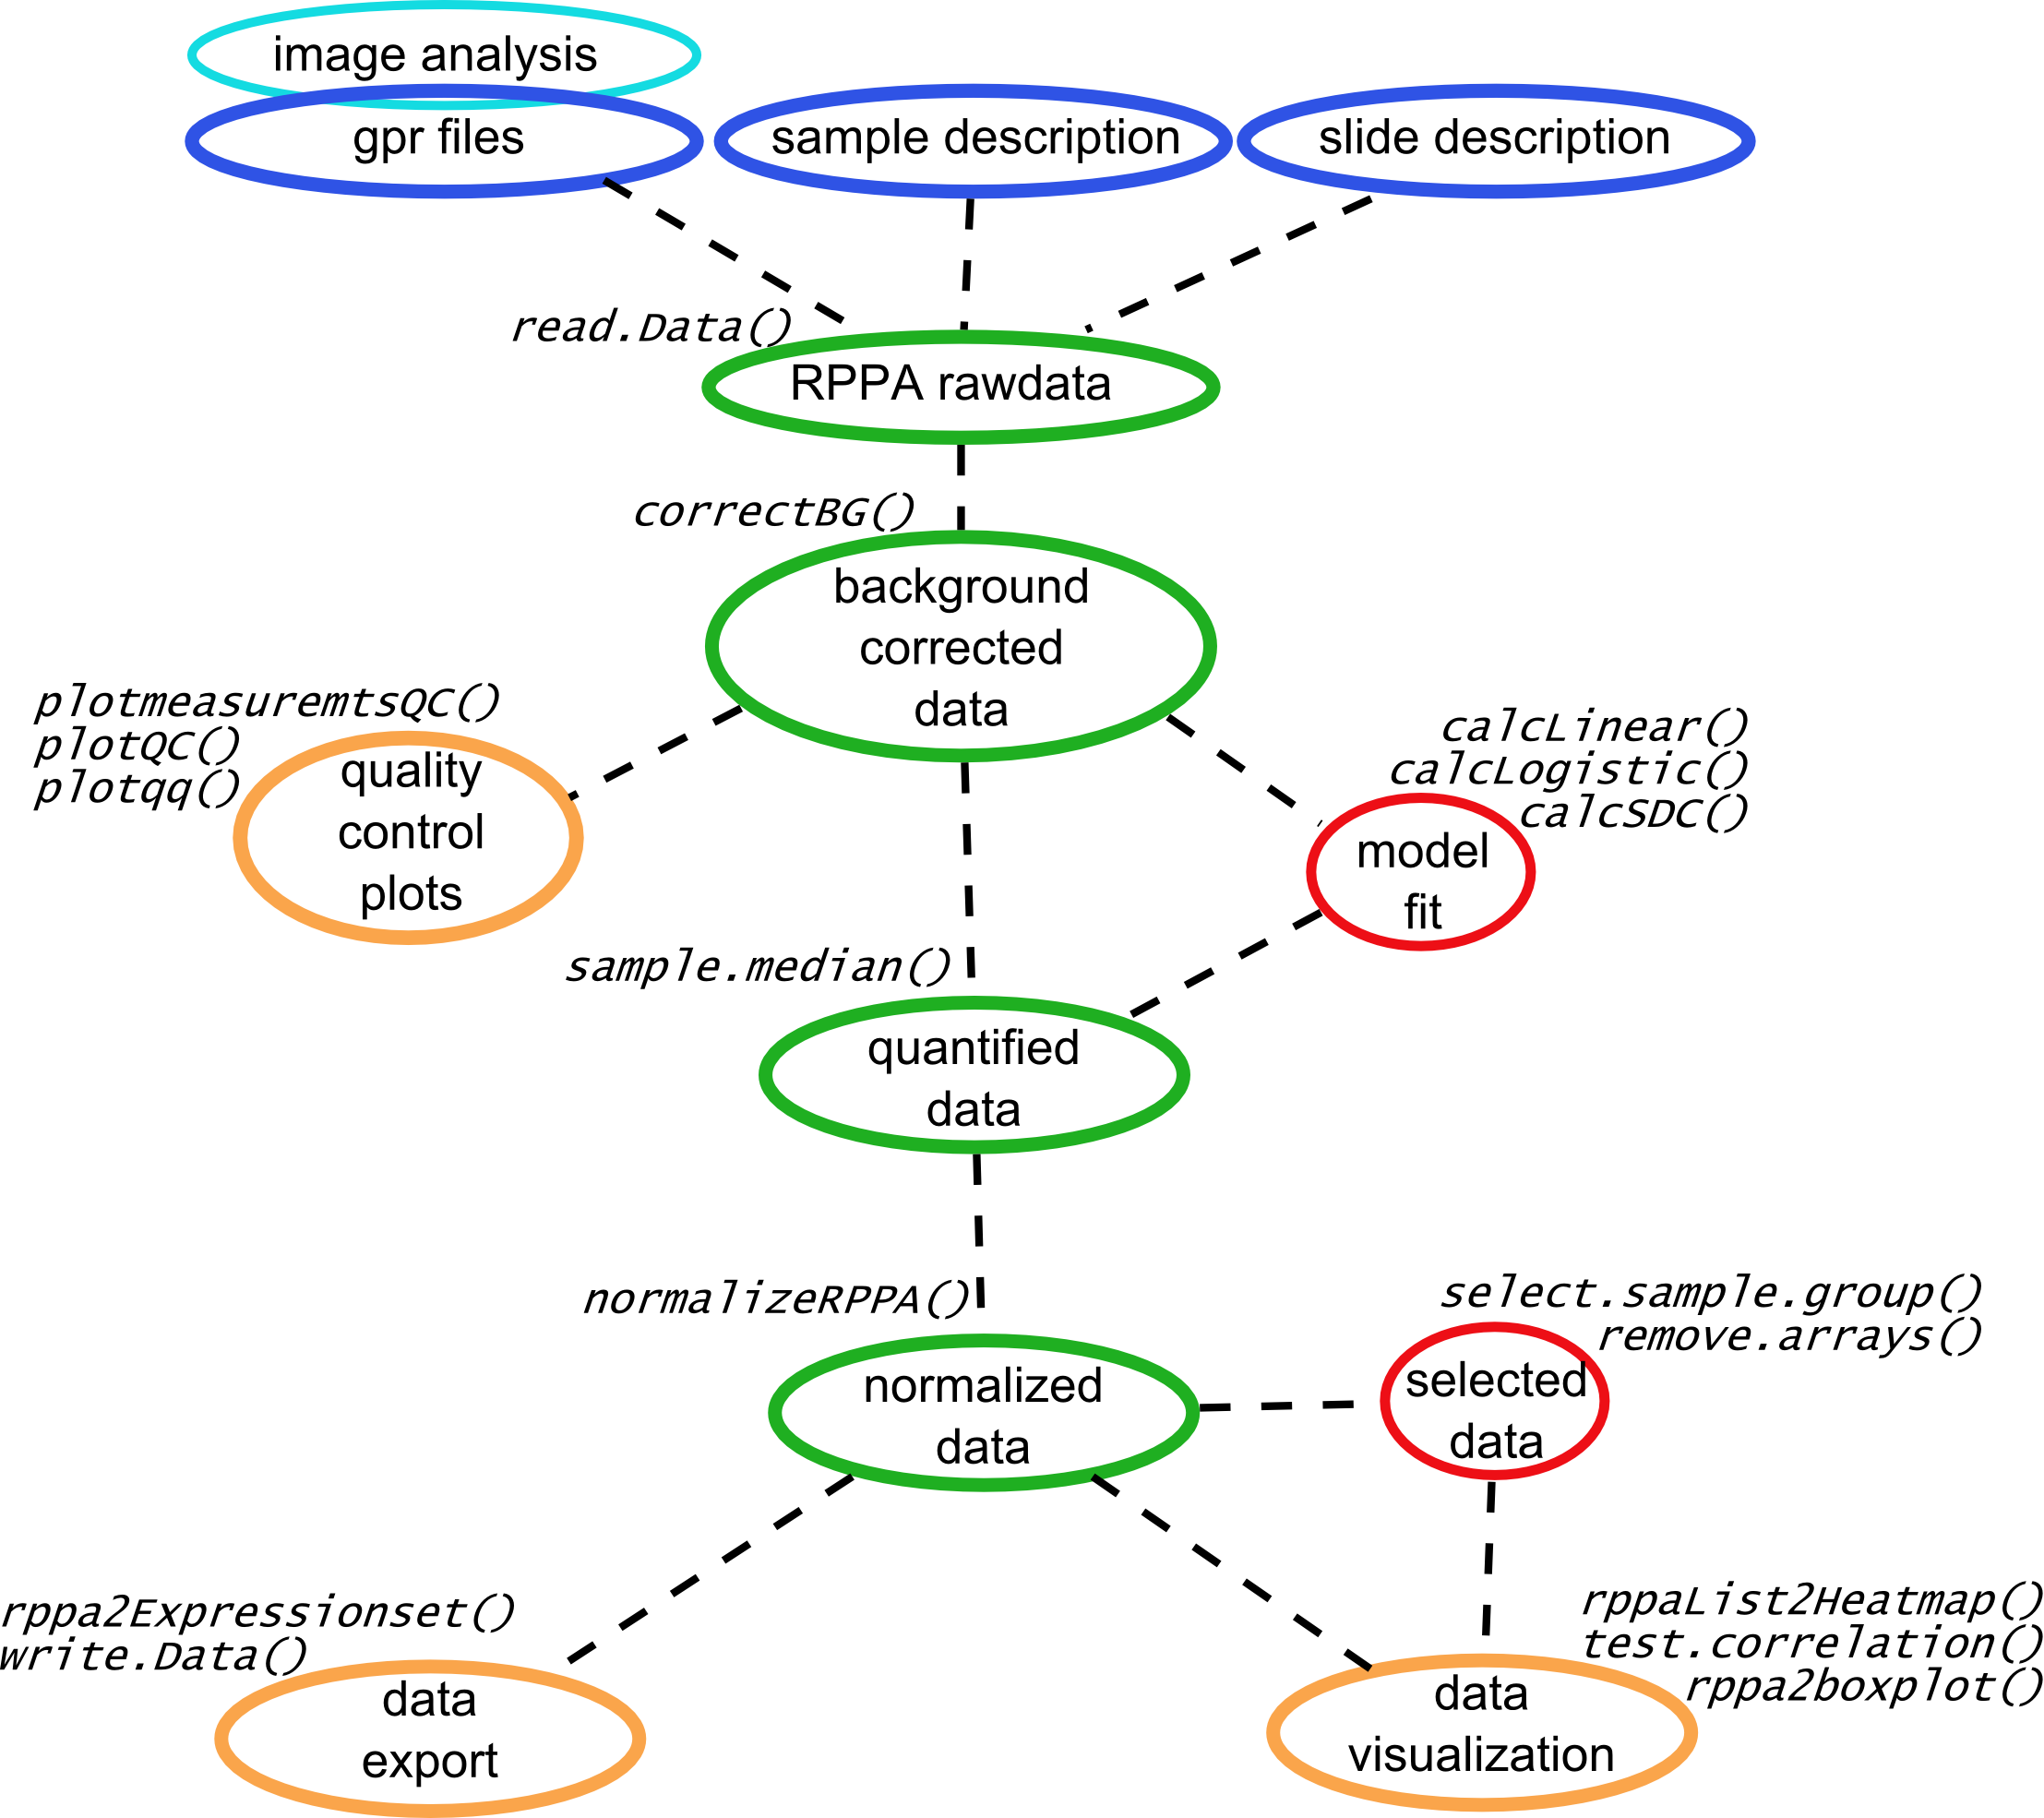
\includegraphics[width=0.7\textwidth]{workflow_RPPanalyzer.png}}
\caption{Workflow for the analysis or reverse phase protein array data using the
RPPanalyzer package}
\label{workflow}
\end{figure}

\section{Data preparation}

To avoid errors during data analysis it is very important to prepare the input data
exactly in the format as described in the following sections. It is not necessary to adjust the
benchwork to the software but to describe exactly what you have done in the lab.


\subsection{Sample description}

Every information concerning the samples has to be stored in a tab delimited
text file and named \texttt{sampledescription.txt} (use spreadsheet software like MS Excel or OOo Spreadsheet to generate the table).
The sample description file contains seven
mandatory columns that are required to identify the samples (described in detail below) and optional columns holding
any information describing the samples in more detail. To select sample groups for
separate analysis it is of advantage to store every type of information in a separate
column. To access example files load the RPPanalyzer package:

\begin{Schunk}
\begin{Sinput}
> library(RPPanalyzer)
\end{Sinput}
\end{Schunk}

An example sample description file describing a serially diluted samples set
is included.

\begin{Schunk}
\begin{Sinput}
> ## define path to example files
> dataDir <- system.file("data",package="RPPanalyzer")
> ## change working directory
> setwd(dataDir)
> ## store example sample description in a variable
> sampledescription <- read.delim("sampledescription.txt")
> ## show sample description header
> head(sampledescription)
\end{Sinput}
\end{Schunk}


\subsubsection{Columns plate, row and column}

These columns describe the location of the samples in the spotting source well plate.
The column \Rfunarg{plate} contains the number of the source well plate stored as an integer (1, 2, 3...).
The Column \Rfunarg{row} contains capital letters (e.g. A-P) and the column \Rfunarg{column} integers (e.g 1-24) to identify the position within one source well plate.

\subsubsection{Column sample\_type}

The column \Rfunarg{sample\_type} holds information about the type of the appropriate sample. Entries ''measurement'' indicate an experimental measurement whereas ''control'' denotes spots for investigation of antibody binding dynamics. Accordingly ''neg\_control'' is reserved for control spots (e.g. BSA) which can be used to investigate unspecific binding. Finally, ''blank'' indicates empty spots (e.g. only buffer).

\subsubsection{Column sample}

Provide an identifier for your samples in this column. It is of advantage to keep this terms unique
in case of clinical samples, for cell culture experiments put in the name of the cell line and
add more columns describing every experimental parameter.

\subsubsection{Columns concentration and dilution}

The column \Rfunarg{concentration} provides numeric data with information of the sample concentration. In case of serially diluted samples describe the dilution steps (starting with a $1$ for the highest concentration) in column \Rfunarg{dilution}.

\subsection{Slide description}

Write all information describing the slides and arrays in a tab delimited text file and name it \texttt{slidedescription.txt}.
Like in the \emph{sampledescription} file seven obligatory columns have to be provided and any optional column can be added.

\begin{Schunk}
\begin{Sinput}
> dataDir <- system.file("data",package="RPPanalyzer")
> setwd(dataDir)
> ## store example sample description in a variable
> slidedescription <- read.delim("slidedescription.txt")
> ## show sample description header
> head(slidedescription)
\end{Sinput}
\end{Schunk}

\subsubsection{Column gpr}

To find the GenePix result files (\emph{gpr} files) in the current folder, the terms stored in the column \Rfunarg{gpr} are used as identifier. That means you have to use exactly identical terms for the names of the \emph{gpr} files and in the \Rfunarg{gpr} column.
If you print multiple arrays on one slide describe the arrays using the same order like on the slide. That means start with describing the uppermost array, than the array below in the next row of the \emph{slidedescription} file) and so on.

\subsubsection{Columns pad, slide, incubation\_run and spotting\_run}

The column \Rfunarg{pad} holds the number of the pad or array on the slides. The column \Rfunarg{slides}
holds the number of the slide. Arrays that were analyzed in parallel are identified
via the \Rfunarg{incubation\_run} column. Make sure that you have exact one blank array (incubated with 2nd antibodies only)
for each incubation run. The column \Rfunarg{spotting\_run} specifies the arrays that were
printed in parallel. You have to provide at least one array with normalizer signals per print run
for the normalization method \Rfunarg{housekeeping}. In case of normalizing using a protein dye (method \Rfunarg{proteinDye}), a whole slide has to be provided.

\subsubsection{Columns target and AB\_ID}

In order to be able to assign the right proteins to the arrays the column \Rfunarg{target} holds the protein name and \Rfunarg{AB\_ID} the corresponding antibody ID. Please use only regular characters (letters, digits, ''\_'', and ''-'').

\subsection{Image analysis result files}

So far the software is restricted to read GenePix result files (\emph{gpr} files). For spot identification grid in the image analysis software (here\: GenePix) use the GenePix array list (\emph{gal} file) that is produced by the spotting device (e.g. Aushon 2470 or ArrayJet).


\section{Read data}

Change to the directory where your data files are stored. This can be done using
the R working menu (File > change directory...) or by using the command \Rfunction{setwd}. Following a little example demonstrating the first steps.
\begin{Schunk}
\begin{Sinput}
> dataDir <- system.file("data",package="RPPanalyzer")
> setwd(dataDir)
\end{Sinput}
\end{Schunk}

The data analysis starts with reading the data from the current working directory.
The argument \Rfunarg{blocksperarray} gives the number of blocks that are printed in one array.
This number is used to separate multiple arrays on one slide that are incubated individually.
With the argument spotter the package takes in account the difference in the column ID which is
used to identify the samples. To get information about the manually flagged spots, set
the printFlags argument to \Rfunarg{TRUE} to export these flags to CSV file.

\begin{Schunk}
\begin{Sinput}
> rawdata <- read.Data(blocksperarray = 4, spotter = "arrayjet",printFlags=FALSE)
\end{Sinput}
\end{Schunk}

After reading the RPPA data an R-object (list with four elements) is created. The first element
holds a matrix with the foreground (expression) intensity data, the second a matrix with background intensities.
The columns of the matrix are representing the individual arrays described by the
third element of the data list, a data frame holding the array information. The rows of the matrix are described by the fourth element holding the sample information.


\section{Correct for background intensities}

To correct for background signals, you can use all methods from the \Rfunction{backgroundcorrect}
functions of the \emph{limma} package \citep{limma} or use the method \Rfunarg{addmin} which subtracts the local background and adds a small constant value to avoid negative signals.

\begin{Schunk}
\begin{Sinput}
> dataBGcorrected <- correctBG(rawdata,method="normexp")
\end{Sinput}
\end{Schunk}

\section{Quantify concentration}

In case of serially diluted samples you have to calculate the (relative) concentration 
of the samples. You can use either a linear model (function \Rfunction{calcLinear}) or a logistic three parameter model (function \Rfunction{calcLogistic}). We recommend to use the Serial Dilution Curve algorithm \cite{Zhang:2009p812} which is the most recent development and produces very robust concentration values (function \Rfunction{calcSdc}). Another possibility of quantification is the \emph{SuperCurve} package \citep{supercurve} which can be accessed using the wrapper function \Rfunction{calcSuperCurve}. 
To use the  \Rfunction{calcSuperCurve} function you have to download and install the package from the MD Anderson Bioinformatics home page (\url{http://bioinformatics.mdanderson.org/Software/OOMPA/}).

\begin{Schunk}
\begin{Sinput}
> ## To run the serial dilution curve algorithm it is neccessary
> ## to aggregate replicate spots first.
> medianValues <- sample.median(dataBGcorrected)
> ## calculate concentration (for the attributes see help pages)
> 
> c_Values <- calcSdc(medianValues,sample.id=c("sample","sample.n"), 
+                     sel = c("measurement", "control"), D0 = 2 )
\end{Sinput}
\end{Schunk}
For the arguments of the \Rfunction{calcSdc} function we want to refer to the help page which can be accessed with
\begin{Schunk}
\begin{Sinput}
> ?calcSdc
\end{Sinput}
\end{Schunk}

\section{Quality control plots}

Signal validity and antibody dynamics can be checked by comparing the target specific signals to the corresponding blank value of the serially diluted control samples (column \Rfunarg{sample\_type} in the \emph{sampledesription} file).
 For this function it is necessary to have one blank array (incubated 
only with secondary antibodies) for each incubation run (column \Rfunarg{incubation\_run} in the 
\emph{slidedescription} file). We included an additional data set containing an
experiment with siRNA transfected cell lines to demonstrate the plotting routines.

\begin{Schunk}
\begin{Sinput}
> ## load data set
> data(HKdata)
\end{Sinput}
\end{Schunk}

\begin{Schunk}
\begin{Sinput}
> plotQC(HKdata,file = "control_samples.pdf",arrays2rm = c("protein"))
\end{Sinput}
\end{Schunk}

Additionally you can plot the blank signals against the target signal of the measurements
(column \Rfunarg{sample\_type} in the sample description file).

\begin{Schunk}
\begin{Sinput}
> plotMeasurementsQC(HKdata,file = "control_measurements.pdf",
+                    arrays2rm = c("protein"))
\end{Sinput}
\end{Schunk}

To check the data distribution for each measured target you can generate a PDF file
with a quantile-quantile plot. This can be done before and after normalization of the data.

\begin{Schunk}
\begin{Sinput}
> plotqq(HKdata,fileName = "qqplot_measurements.pdf")
\end{Sinput}
\end{Schunk}

\section{Data normalization}

Normalization is a crucial step in RPPA data analysis to ensure sample comparability and to yield 
high quality data. The reference value to normalize RPPA is the total protein amount per spot.
There are different possibilities to generate this reference value that will be described in detail below. 
The following signal normalization steps can be applied directly to background corrected data if the samples are spotted in only one concentration. For serially diluted samples the normalization step is performed on the quantified data. Otherwise the information of the signal dynamics in one dilution series is lost.

\subsection{Total protein dyes}

The most common method to normalize RPPA data is to stain one slide representative 
for one print run with a total protein dye like Fast Green FCF (see also \cite{Loebke:2007p612})
or Sypro Ruby or colloidal Gold (see also \cite{Spurrier:2008p934}). 

After calculating the $log_2$ intensities the normalizer value can simply subtracted from the target signal to obtain the \emph{relative protein expression}. In case of multiple arrays on one slide  the normalization is working array wise (pad wise). That means each array is normalized by the corresponding array on the normalizer slide. The normalization method \Rfunarg{proteinDye} requires one normalizer slide per print run and will be identified as ''protein'' in the \Rfunarg{target} column of the \emph{slidedescription} file. If you want to obtain values in native scale (instead of $log_2$ scale) you have to change the \Rfunarg{vals} attribute to ''native''.

\begin{Schunk}
\begin{Sinput}
> norm_values_pd <- normalizeRPPA(HKdata,method="proteinDye",vals="logged")
\end{Sinput}
\end{Schunk}

\subsection{Housekeeping proteins}
Proteins that are expected to be expressed at a constant level, not effected by the 
experimental conditions, can be used as housekeeping proteins for normalization. This
method is established for quantitative Western blots and can be utilized to normalize RPPA. 
To obtain the normalizer value, the mean of all arrays identified with the ''normalizer'' 
attribute (column \Rfunarg{target} in the \emph{slidedescription} file) is calculated within one print run. 

\begin{Schunk}
\begin{Sinput}
> norm_values_hk <- normalizeRPPA(HKdata,method="housekeeping",
+                              normalizer="housekeeping",vals="logged")
\end{Sinput}
\end{Schunk}

In case of a fluorescent readout it is possible to incubate antibodies against housekeeping proteins after the target
specific antibodies and label them for detection at a different wavelength. Using this approach it is
possible to generate the normalizer signal from the same spot as the target specific signal. This
enables to correct for spotting imprecisions that could not be identified on just one (or a few) representative
slides per print run.

\begin{Schunk}
\begin{Sinput}
> norm_values_hk_sbs <- normalizeRPPA(HKdata,method="spotbyspot",
+                              normalizer="housekeeping",vals="logged")
\end{Sinput}
\end{Schunk}

\subsection{Median normalization}

Assuming that all proteins measured in the RPPA experiment are reflecting the total protein amount this can be used
as a normalizer value. The median value of all protein signals of each spot or sample is calculated and used as normalizer signal. 

\begin{Schunk}
\begin{Sinput}
> norm_values_row <- normalizeRPPA(HKdata,method="row")#,vals="logged")
\end{Sinput}
\end{Schunk}

  
\subsection{Protein quantification assays}

The method \Rfunarg{extValue} provides the possibility to utilize protein concentration values 
determined with protein quantification assays (e.g. Bradford, BCA) as normalizer value. 
The protein concentration has to be provided in a column in the sample description 
file and will be accessed with the attribute \Rfunarg{useCol}. This method needs very precise spotting device
since the value does not include spotting imprecisions.

\begin{Schunk}
\begin{Sinput}
> norm_values_eV <- normalizeRPPA(HKdata,method="extValue",
+                              useCol="concentration",vals="logged")
\end{Sinput}
\end{Schunk}

\begin{Schunk}
\begin{Sinput}
> ## all normalization method were performed on a sample set that was spotted in
> ## replicates (not serially diluted). In this case you can aggregate the replicate
> ## spots after the normalization:
> norm_data <- sample.median(norm_values_pd)
\end{Sinput}
\end{Schunk}

\section{Export data as text file}
   
It is possible to export the RPPA data set as tab delimited text file at any point 
during data analysis for further inspection using spreadsheet software. The data will 
be stored in two files, representing the expression and background or expression and 
error, depending on the analysis step. The rows of the table will be annotated with sample
information, the columns with array information.

\begin{Schunk}
\begin{Sinput}
> write.Data(norm_data,FileNameExtension="test_data")
\end{Sinput}
\end{Schunk}

The text files will be stored in the current working directory.

\section{Array and data selection}

To select a sample group of interest for further analysis it is possible to access 
the samples using any column (attribute \Rfunarg{params}) of the \emph{sampledecription} and define
the samples of interest (attribute \Rfunarg{sel}).

\begin{Schunk}
\begin{Sinput}
> selectedSamples  <-  select.sample.group(norm_data,
+                      params=list("replicate"=c("1")))
\end{Sinput}
\end{Schunk}

Furthermore, it is possible to exclude arrays from further analysis which you have identified as not valid or
not necessary. They will be identified using the \Rfunarg{target} information in the \emph{slidedescription} file.

\begin{Schunk}
\begin{Sinput}
> selectedData <-   remove.arrays(selectedSamples,param="target",
+                   arrays2rm=c("protein", "blank","housekeeping"))
\end{Sinput}
\end{Schunk}

\section{Visualizations}

RPPanalyzer provides several standard visualization tools to get an overview of
the biological relevance of the data set.


\subsection{Time courses}

RPPAs allow the measurement of the phosporylation status of proteins. Therefore they capacitate, in contrast to mRNA based techniques, to investigate signaling pathways in a time resolved manner. Such time course experiments can be visualized with the plotTimeCourse function.

The function will generate a PDF in the current working directory. The argument \Rfunarg{tc.identifier} combines the sample attributes which will identify the individual time course experiments whereas the \Rfunarg{plot.split} argument will be used to define which time course experiments will be plotted in one graph. The argument \Rfunarg{plotformat} defines the way the data will be plotted: ''rawdata'' will plot the time points connected with dashed lines, ''splines'' will plot a smoothed spline calculated using the package \emph{gam} \citep{gam}. To plot both set \Rfunarg{plotformat} to ''both''.

\begin{Schunk}
\begin{Sinput}
> ## load a time course data set
> data(dataII)
> plotTimeCourse(dataII,
+ tc.identifier = c("sample","stimulation","inhibition","stim_concentration"),
+ #tc.reference = NULL,
+ plot.split = "experiment", file = "Timeplot.pdf",
+ arrays2rm = c("protein", "Blank"), plotformat = "spline")
\end{Sinput}
\end{Schunk}

\subsection{Boxplots}

The (differential) expression of proteins between distinct groups can be visualized in boxplots.
To calculate the p-value associated with a test on differences, you have to define a control within the parameter you want to plot. A PDF is generated and saved in the current working directory.

\begin{Schunk}
\begin{Sinput}
> ## load data set
> data(dataIII)
> ## normalize data
> n.data <- normalizeRPPA(dataIII,method="row")
> ## aggregate replicates
> cl.data <- sample.median(n.data)
> ## draw boxplots and generate PDF
> rppa2boxplot(cl.data,param = "tissue", wilcoxtest = TRUE,
+             control = "A",file = "boxplot_groups.pdf")
\end{Sinput}
\end{Schunk}

\subsection{Correlation plots}

If you want to correlate the protein expression or phosphorylation status to numeric sample attributes,
you can use the \Rfunction{test.correlation} function (a wrapper for \Rfunction{cor.test}). Define the correlation method with the\Rfunarg{method.cor} argument and the method to correct the p-values for multiple testing in \Rfunarg{method.padj}. A PDF will be generated in the current working directory.

\begin{Schunk}
\begin{Sinput}
> test.correlation(cl.data,
+             param = "concentration",method.cor = "kendall",
+             method.padj = "BH", file = "correlation_plot.pdf")
\end{Sinput}
\end{Schunk}

\subsection{Heatmaps}

A common method to present high dimensional biological data are heatmaps. The RPPanalyzer provides a function to plot heatmaps annotated with any sample attribute in order to check if the sample attribute corresponds to the clustering. Thereby the parameter \Rfunarg{sampledesription} defines which information is used for grouping the samples. To ensure a stable and meaningful clustering removing control arrays and arrays of bad quality is recommended preceding step.

\begin{Schunk}
\begin{Sinput}
> ## remove some arrays
> sel.data <- remove.arrays(cl.data,param="target",
+             arrays2rm=c("target10","target2","target21","target22",
+             "target28","target33","target36","target38","target61",
+             "target47","target13","target19"))
> rppaList2Heatmap(sel.data,
+       sampledescription = "sample",side.color = "tissue",
+       remove = c("blank", "protein", "Abmix"), distance = "euclidean",
+       dendros = "both", cutoff = 0.005, fileName = "Heatmap.pdf",
+       cols = colorpanel(100, low = "blue", mid = "yellow", high = "red"))
\end{Sinput}
\end{Schunk}

\bibliographystyle{abbrvnat}
\bibliography{papers_RPPanalyzer}

\end{document}
